\chapter{ANTECEDENTES.} % (((

\section{DATOS GENERALES.} % (((
\begin{tabular}{r @{\bf : \hspace{5mm}} p{0.7 \linewidth}}
	\bf Soicitante del avalúo & \personaSolicitante. \\ 
	\bf Propietario           & \nombrePropietario \\ 
	\bf Fecha del avalúo      & \fechaInforme. \\ 
	\bf Valuador              & \peritoValuador. \\ 
	\bf Especialidad          & \tipoAvaluo. \\ 
	\bf Bienes que se valúan  & \bienesValuados. \\ 
	\bf Objeto del avalúo     & \objetoValuacion. \\ 
	\bf Propósito del avalúo  & \propositoValuacion. \\ 
	\bf Fecha de Inspeccion   & \fechaInspeccion. \\ 
	\bf Fecha de Reporte      & \fechaInforme. \\ 
	\bf Condición             & \condicionAvaluo. \\ 
	\bf C. Responsable        & \cResponsable. \\ 
	\bf Sucursal              & \sucursal. \\ 
	\bf Cédula Profesional    & \cedulaProfesional
\end{tabular}
% )))

\section{UBICACIÓN DE LOS BIENES A VALUAR.} % (((
\begin{tabular}{r @{\bf : \hspace{5mm}} p{0.25 \linewidth}}
	\bf Calle         & \calle. \\ 
	\bf No. Exterior  & \numExterior. \\ 
	\bf Colonia       & \colonia. \\ 
	\bf Municipio     & \municipio. \\ 
	\bf Código Postal & \codigoPostal.
\end{tabular}
\begin{tabular}{r @{\bf : \hspace{5mm}} p{0.25 \linewidth}}
	\bf No. Interior       & \numInterior. \\ 
	\bf Población o Ciudad & \ciudad. \\ 
	\bf Entidad Federativa & \entidadFederativa.
\end{tabular}
% )))

\section{CROQUIS DE UBICACIÓN DE LOS BIENES.} % (((
\begin{figure}[hbtp!]
	\centering
	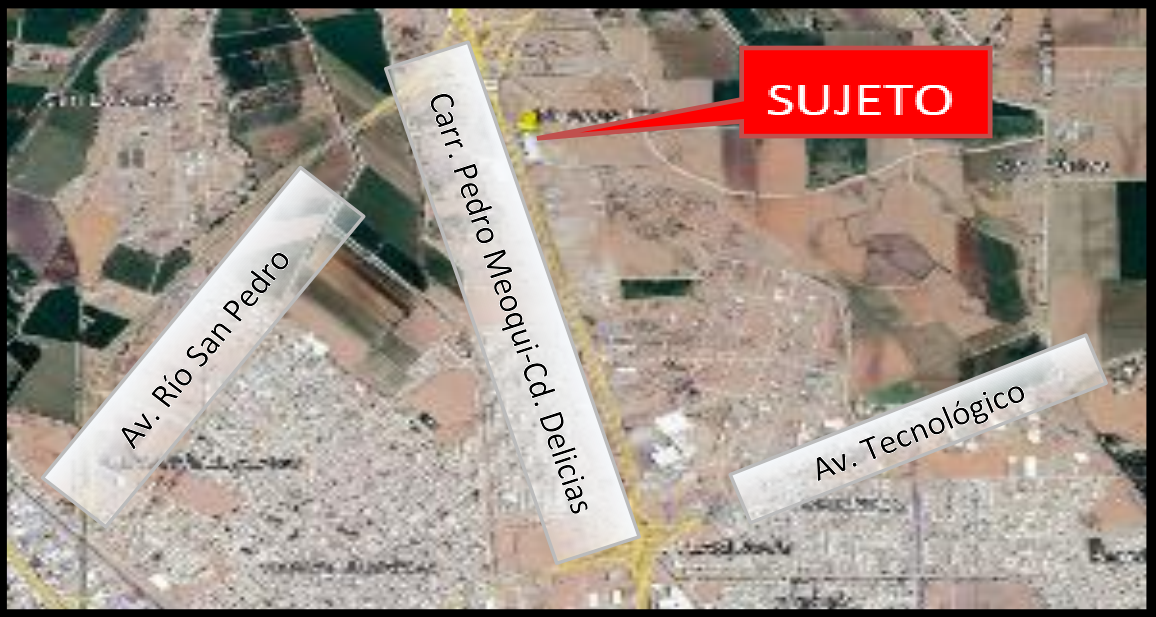
\includegraphics[width= 0.4 \linewidth, page = 1]{../0.imagenes/CAP_1/1}
	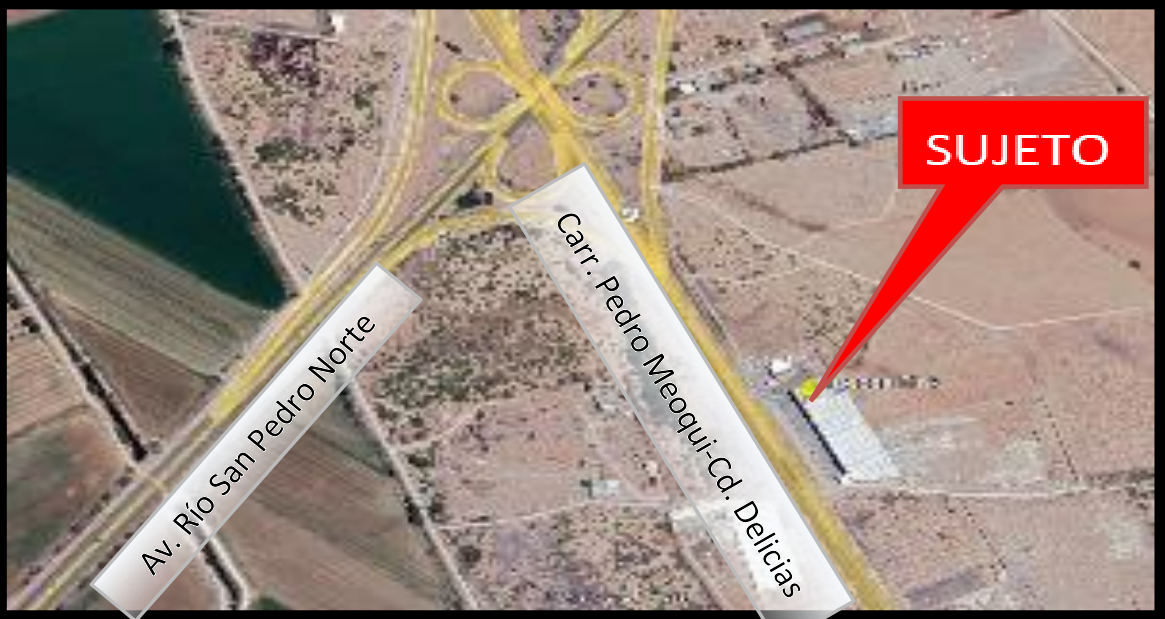
\includegraphics[width= 0.4 \linewidth, page = 1]{../0.imagenes/CAP_1/2}
\end{figure}
\textbf{Georeferencias:} \\[2mm]
\hfill 
\textbf{Latitud:} \latitud
\hfill 
\textbf{Longitud:} \longitud
\hfill 
\textbf{Altitud:} \altitud
\hfill 
% )))

% )))
